\begin{exercise}{0}

  \begin{subexercise}
    \emph{Pig} is a high level scripting language that is used with Apache Hadoop. Pig enables data workers to write complex data transformations without knowing Java. Pig’s simple SQL-like scripting language is called Pig Latin, and appeals to developers already familiar with scripting languages and SQL.
    Apache Hive is an open source data warehouse system for querying and analyzing large data sets that are principally stored in Hadoop files. The users are provided with strong and powerful statistics functions with hive and It is similar to SQL and hence it is very easy to understand the concepts.

    So, we can say that, the main goal of high level languages like pig or hive is to reduce the workload of the user by preventing the need of writing complex map-reduce jobs in java or python.
  \end{subexercise}
  
  \begin{subexercise}
    Whenever we do a groupBy or groupByKey on a RDD We typically move data from one node to another to be grouped with its key. Doing this is called Shuffling. We need shuffling, when a distribution of RDD between different nodes of a cluster cannot be performed within a single partition. Examples of such operations are join, distinct, groupByKey. 
    When a partition is dependent of one or two parent partitions it is called "Narrow dependencies". And when a partition is dependent on multiple parent partitions it is called "wide dependencies".
  \end{subexercise}
  
  \begin{subexercise}
    Mediator is an approach to data integration, it acts as an intermediate medium transforming queries to sub-queries, integrating result data and resolving conflict. It maintains a global schema and mappings between the global and source schemas. It is the task of the mediator to consult the mappings to decide which data to retrieve from the sources and how to combine them appropriately in order to form the answer to the user's query. \\
    \centering
    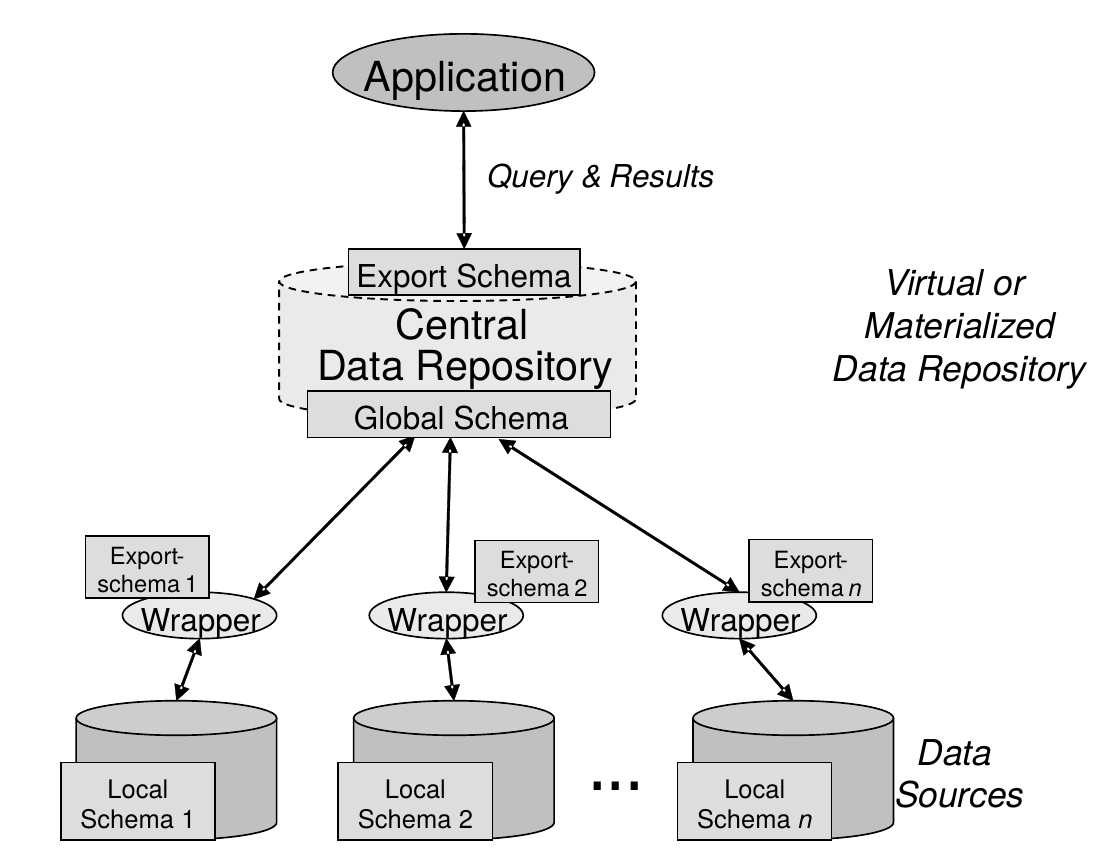
\includegraphics[width=0.5\textwidth]{ueb06/image.png}
  \end{subexercise}
  
  \begin{subexercise}
    Herbrand Base of D: All positive ground literals are constructable from predicates in D and constants in D.
    Herbrand Model of D: A Herbrand Model is every subset M of the Herbrand Base of D, such that: Every fact from F is contained in M. For every ground instance of a rule in D over constants in D, if M contains all literals in the body, then M contains the head as well. A minimal model does not properly contain any other model 
  \end{subexercise}

\end{exercise}
